%
\documentclass[english]{../thermomemo/thermomemo}

\usepackage{textcomp}
\usepackage{natbib}
\usepackage{amsmath}
%\usepackage{pslatex}
%\usepackage{bm}% better \boldsymbol
\usepackage{array}% improves tabular environment.
\usepackage{dcolumn}% also improves tabular environment, with decimal centring.
\usepackage{lastpage}
%\usepackage{listings}
\usepackage{tikz}
\usepackage{pgfplots}
\usepackage{cleveref}
\usepackage{pgf,pgfarrows,pgfnodes}
\usepackage{enumerate}
\usepackage[final]{pdfpages}
\usepackage[altbullet,expert]{lucidabr}
%\usepackage[charter]{mathdesign}

\usepackage{ifthen}
\usepackage{nomencl}
\usepackage{parskip}
\usepackage{psfrag}
\usepackage{pstool}
\usepackage{booktabs}
\usepackage{pifont}
%\usepackage{subfig,caption}
\usepackage{microtype}% for pdflatex; medisin mot overfull \vbox
\usepackage{subcaption,caption}
\usepackage{mhchem}
\usepackage{siunitx}
\usepackage{todonotes}
\presetkeys{todonotes}{inline}{}

\usepackage{xcolor}
\hypersetup{
  colorlinks,
  linkcolor={red!50!black},
  citecolor={blue!50!black},
  urlcolor={blue!80!black}
}

\newcommand*{\checked}{\ding{51}}
\graphicspath{{data/}}
%% Formattering av figur- og tabelltekster
%
% Std. fra KOMA. Koplet ut pga. subfig:
%\setkomafont{caption}{\normalfont\normalsize\sffamily}
%\setkomafont{captionlabel}{\normalfont\normalsize\sffamily}
% eventuelt \setcapindent{0cm} hvis man ikke vil ha �hanging caption�
% Vil ikke ha dot (`Figure 1.1.:' er teit):
%\renewcommand*{\figureformat}{\figurename~\thefigure}%\autodot
%\renewcommand*{\tableformat}{\tablename~\thetable}%\autodot
%
% Caption (og alt):
\captionsetup{labelfont=sf,textfont=sf,format=hang}
% like option tablecaptionabove to KOMA-script
\captionsetup[table]{position=top}
% Subfig:
% (Hack;
% http://groups.google.com/group/comp.text.tex/browse_thread/thread/7de1c7c60103c79/d920432878a413d0?lnk=st&q=subfig+ref+group%3Acomp.text.tex&rnum=2&hl=en#d920432878a413d0) (Vilar Camara Neto)
%\captionsetup[subfloat]{labelformat=simple,listofformat=subsimple} 
%\renewcommand*{\thesubfigure}{(\alph{subfigure})}
%
% Shorthand for figure inclusion:
\newcommand*{\stmfig}[4]{%width,name,xlabel,ylabel
\parbox[t]{#1}{%
  \makebox[0pt][l]{\small#4}\\[-0.8\baselineskip]%
  \parbox[b]{#1}{\includegraphics[width=#1]{#2}%
    \makebox[0pt][r]{\raisebox{0.0mm}[0pt][0pt]{\small#3}}%
  \rule[-2.0mm]{0pt}{0pt}}}}
%
% Formattering av lister ??
% \renewcommand*{\labelitemi}{\textthreequartersemdash}
% \renewcommand*{\labelitemii}{$\circ$}
% \renewcommand*{\labelitemiii}{\textasteriskcentered}
% \renewcommand*{\labelitemiv}{\textperiodcentered}
%
% Kolonnetyper for array.sty:
\newcolumntype{C}{>{$}c<{$}}% for � slippe � taste inn disse $
\newcolumntype{L}{>{$}l<{$}}% for � slippe � taste inn disse $
% For dcolumn.sty
\newcolumntype{d}[1]{D{.}{.}{#1}}
%
% Egendefinerte
%
\newcommand*{\unit}[1]{\ensuremath{\,\mathrm{#1}}}
\newcommand*{\uunit}[1]{\ensuremath{\mathrm{#1}}}
%\newcommand*{\od}[3][]{\frac{\mathrm{d}^{#1}#2}{\mathrm{d}{#3}^{#1}}}% ordinary derivative
\newcommand*{\od}[3][]{\frac{\dif^{#1}#2}{\dif{#3}^{#1}}}% ordinary derivative
\newcommand*{\pd}[3][]{\frac{\partial^{#1}#2}{\partial{#3}^{#1}}}% partial derivative
\newcommand*{\pdt}[3][]{{\partial^{#1}#2}/{\partial{#3}^{#1}}}% partial
                                % derivative for inline use.
\newcommand{\pone}[3]{\frac{\partial #1}{\partial #2}\bigg|_{#3}}% partial
                                % derivative with information of
                                % constant variables
\newcommand{\ponel}[3]{\frac{\partial #1}{\partial #2}\bigg|_{#3}} % partial derivative with information of constant variable. A line is added.
\newcommand{\ptwo}[3]{\frac{\partial^{2} #1}{\partial #2 \partial
    #3}} % partial differential in two different variables
\newcommand{\pdn}[3]{\frac{\partial^{#1}#2}{\partial{#3}^{#1}}}% partial derivative

% Total derivative:
\newcommand*{\ttd}[2]{\frac{\mathrm{D} #1}{\mathrm{D} #2}}
\newcommand*{\td}[2]{\frac{\mathrm{d} #1}{\mathrm{d} #2}}
\newcommand*{\ddt}{\frac{\partial}{\partial t}}
\newcommand*{\ddx}{\frac{\partial}{\partial x}}
% Vectors etc:
% For Computer Modern:

\DeclareMathAlphabet{\mathsfsl}{OT1}{cmss}{m}{sl}
\renewcommand*{\vec}[1]{\boldsymbol{#1}}%
\newcommand*{\vektor}[1]{\boldsymbol{#1}}%
\newcommand*{\tensor}[1]{\mathsfsl{#1}}% 2. order tensor
\newcommand*{\matr}[1]{\tensor{#1}}% matrix
\renewcommand*{\div}{\boldsymbol{\nabla\cdot}}% divergence
\newcommand*{\grad}{\boldsymbol{\nabla}}% gradient
% fancy differential from Claudio Beccari, TUGboat:
% adjusts spacing automatically
\makeatletter
\newcommand*{\dif}{\@ifnextchar^{\DIfF}{\DIfF^{}}}
\def\DIfF^#1{\mathop{\mathrm{\mathstrut d}}\nolimits^{#1}\gobblesp@ce}
\def\gobblesp@ce{\futurelet\diffarg\opsp@ce}
\def\opsp@ce{%
  \let\DiffSpace\!%
  \ifx\diffarg(%
    \let\DiffSpace\relax
  \else
    \ifx\diffarg[%
      \let\DiffSpace\relax
    \else
      \ifx\diffarg\{%
        \let\DiffSpace\relax
      \fi\fi\fi\DiffSpace}
\makeatother
%
\newcommand*{\me}{\mathrm{e}}% e is not a variable (2.718281828...)
%\newcommand*{\mi}{\mathrm{i}}%  nor i (\sqrt{-1})
\newcommand*{\mpi}{\uppi}% nor pi (3.141592...) (works for for Lucida)
%
% lav tekst-indeks/subscript/pedex
\newcommand*{\ped}[1]{\ensuremath{_{\text{#1}}}}
% h�y tekst-indeks/superscript/apex
\newcommand*{\ap}[1]{\ensuremath{^{\text{#1}}}}
\newcommand*{\apr}[1]{\ensuremath{^{\mathrm{#1}}}}
\newcommand*{\pedr}[1]{\ensuremath{_{\mathrm{#1}}}}
%
\newcommand*{\volfrac}{\alpha}% volume fraction
\newcommand*{\surften}{\sigma}% coeff. of surface tension
\newcommand*{\curv}{\kappa}% curvature
\newcommand*{\ls}{\phi}% level-set function
\newcommand*{\ep}{\Phi}% electric potential
\newcommand*{\perm}{\varepsilon}% electric permittivity
\newcommand*{\visc}{\mu}% molecular (dymamic) viscosity
\newcommand*{\kvisc}{\nu}% kinematic viscosity
\newcommand*{\cfl}{C}% CFL number

\newcommand*{\cons}{\vec U}
\newcommand*{\flux}{\vec F}
\newcommand*{\dens}{\rho}
\newcommand*{\svol}{\ensuremath v}
\newcommand*{\temp}{\ensuremath T}
\newcommand*{\vel}{\ensuremath u}
\newcommand*{\mom}{\dens\vel}
\newcommand*{\toten}{\ensuremath E}
\newcommand*{\inten}{\ensuremath e}
\newcommand*{\press}{\ensuremath p}
\renewcommand*{\ss}{\ensuremath a}
\newcommand*{\jac}{\matr A}
%
\newcommand*{\abs}[1]{\lvert#1\rvert}
\newcommand*{\bigabs}[1]{\bigl\lvert#1\bigr\rvert}
\newcommand*{\biggabs}[1]{\biggl\lvert#1\biggr\rvert}
\newcommand*{\norm}[1]{\lVert#1\rVert}
%
\newcommand*{\e}[1]{\times 10^{#1}}
\newcommand*{\ex}[1]{\times 10^{#1}}%shorthand -- for use e.g. in tables
\newcommand*{\exi}[1]{10^{#1}}%shorthand -- for use e.g. in tables
\newcommand*{\nondim}[1]{\ensuremath{\mathit{#1}}}% italic iflg. ISO. (???)
\newcommand*{\rey}{\nondim{Re}}
\newcommand*{\acro}[1]{\textsc{\MakeLowercase{#1}}}%acronyms etc.

\newcommand{\nto}{\ensuremath{\mbox{N}_{\mbox{\scriptsize 2}}}}
\newcommand{\chfire}{\ensuremath{\mbox{CH}_{\mbox{\scriptsize 4}}}}
%\newcommand*{\checked}{\ding{51}}
\newcommand{\coto}{\ensuremath{\text{CO}_{\text{\scriptsize 2}}}}
\newcommand{\celsius}{\ensuremath{^\circ\text{C}}}
\newcommand{\clap}{Clapeyron~}
\newcommand{\subl}{\ensuremath{\text{sub}}}
\newcommand{\spec}{\text{spec}}
\newcommand{\sat}{\text{sat}}
\newcommand{\sol}{\text{sol}}
\newcommand{\liq}{\ensuremath{\ell}}
\newcommand{\vap}{\text{g}}
\newcommand{\amb}{\text{amb}}
\newcommand{\tr}{\text{tr}}
\newcommand{\crit}{\text{crit}}
\newcommand{\entr}{\ensuremath{\text{s}}}
\newcommand{\fus}{\text{fus}}
\newcommand{\mix}{\text{m}}
\newcommand{\flash}[1]{\ensuremath{#1\text{-flash}}}
\newcommand{\spce}[2]{\ensuremath{#1\, #2\text{ space}}}
\newcommand{\spanwagner}{\text{Span--Wagner}}
\newcommand{\fiveeq}{\text{five--equation}}
\newcommand{\twofluid}{\text{two--fluid model}}
\newcommand{\vapliq}{\text{gas--liquid}}
\newcommand{\kk}{\text{k}}
\newcommand{\force}{\text{FORCE}}
\newcommand{\lf}{\text{LF}}
\newcommand{\lw}{\text{LW}}
\newcommand{\rlaxw}{\text{Richtmyer Lax--Wendroff}}
\newcommand{\laxw}{\text{Lax--Wendroff}}
\newcommand{\laxf}{\text{Lax--Friedrichs}}
\newcommand{\loc}{\text{loc}}
\newcommand{\interf}{\text{i}}
\newcommand{\toumi}{\text{Toumi's shock tube}}
\newcommand{\nstar}{{\ensuremath{\text{n}^\ast}}}
\newcommand{\sph}{\text{SP}}
\newcommand{\NR}{\text{Newton-Raphson}}
\newcommand{\res}{\text{R}}
\newcommand{\ideal}{\text{Id}}

% Grid indices
\newcommand{\jj}{j}
\newcommand{\jph}{{j+1/2}}
\newcommand{\jmh}{{j-1/2}}
\newcommand{\jp}{{j+1}}
\newcommand{\jm}{{j-1}}
\newcommand{\nn}{n}
\newcommand{\nph}{{n+1/2}}
\newcommand{\nmh}{{n-1/2}}
\newcommand{\np}{{n+1}}
\newcommand{\mm}{m}
\newcommand{\mph}{{m+1/2}}
\newcommand{\mmh}{{m-1/2}}
\newcommand{\mpp}{{m+1}}
\newcommand{\MM}{M}
\newcommand{\NN}{N}

\graphicspath{{gfx/}}

\title{Thermodynamic equilibrium algorithms - Reimplemented
  in a new framework.}
\author{Morten Hammer}
\usepackage{isodate}
\date{\today}

% Nomenclature groups
\RequirePackage{ifthen}
\renewcommand{\nomgroup}[1]{%
  \ifthenelse{\equal{#1}{A}}{\item[\textbf{Latin letters}]}{%
  \ifthenelse{\equal{#1}{G}}{\item[\textbf{Greek letters}]}{%
  \ifthenelse{\equal{#1}{Z}}{\item[\textbf{Abbreviations and dimensionless numbers}]}{%
  \ifthenelse{\equal{#1}{M}}{\item[\textbf{Vectors and Matrices}]}{%
  \ifthenelse{\equal{#1}{O}}{\item[\textbf{Other symbols and labels}]}{
%
  \ifthenelse{\equal{#1}{S}}{\item[\textbf{Subscripts and superscripts
}]}{}}}{}}}}}
% Spacing
\setlength{\nomitemsep}{-\parsep}
\makenomenclature


\begin{document}
\frontmatter
\tableofcontents
\printnomenclature

\section{Introduction}

In the project \coto~Dynamics, the overall aim is to provide knowledge
about safe and efficient design and operation of \coto-pipeline
transport and injection systems. To achieve this, models capable of
predicting the thermophysical properties of multiphase \coto-mixtures
are needed. Since evaluation of transient \coto-pipeline operation is
made with fluid dynamical models connected to thermodynamic models and
phase-calculations, a high degree of robustness and accuracy is
necessary for numerical stability. State-of-the-art algorithms are
thus needed for the phase calculations. Another reason to implement
the best routines for phase-calculations is the need of a flexible
framework capable of handling multiple liquid-phases and solids such
as dry-ice. The latest algorithms proposed by \cite{Michelsen2007} 
have been implemented as part of the development of the
new flexible workbench for thermodynamics, called ThermoPack,
documented in the Memo DA1201. The underlying equations and algorithms
used to solve the phase equilibrium between two-phase vapour and liquid
with specified temperature and pressure (\flash{TP}), specified
enthalpy and pressure (\flash{HP}) and specified entropy and pressure
(\flash{SP}) will be described.

Many systems in CCS contain several phases. \cite{Austegard2006} for instance, investigated thermodynamic models for
H$_2$O-\coto-CH$_4$ mixtures. In their Fig. 8, for the system
H$_2$O-\coto-CH$_4$ at 298K, a three-phase system occurs between 70-72 bar in
which one water rich liquid-phase forms, one \coto~rich liquid-phase
forms and a CH$_4$ rich vapour-phase is formed. To be able to predict
when a \coto-rich system will consist of several liquid-phases and
also to calculate the composition of them, a multiphase flash routine
has been implemented in ThermoPack. In this memo, it will be shown
that the implementation can successfully predict phase-diagrams with
more than one liquid phase for two relevant mixtures.

All the code has been implemented in a Fortran 90$/$95-syntax and a
Mercurial version control has been used to track changes and merge the
developments in the source-code of ThermoPack. The same test
functionality in the COTT-code developed in Task B and C of this
project has been used to test the code. To have an active and
up-to-date documentation, comments have been added in a syntax used by
the popular program Doxygen. The algorithms and equations used may be
found in Section \ref{sec:algorithms}. Results from tests and comparisons are located in
Section \ref{sec:results}, while conclusions and suggestions for further work can be
found in Section \ref{sec:conclusion}.

\section{Algorithms and equations}
\label{sec:algorithms}
\subsection{Chemical potential}
Chemical potential, $\mu$, of a fluid, i, with composition $z_{\text{i}}$, is given by the following equation,
\begin{align}
  \pd{G}{n_{\text{i}}} = \mu_{\text{i}} &=\mu_{\text{i}}^0 + RT \ln \biggl(\frac{f_{\text{i}}}{P^0}\biggr)\\
  f_{\text{i}} &= z_{\text{i}} \varphi_{\text{i}} P
\label{eq:chempot}
\end{align}
Where $f$ is the fugacity and $\varphi$ is the fugacity factor.

\subsection{Wilson-K factors}
Wilson-K factors are used as initial values in the \flash{TP}, and are given as
\begin{equation}
  K_{\text{i}}^{Wilson} = \frac{P^c_{\text{i}}}{P}\exp \biggl(5.373 (1+\omega_{\text{i}})
  \biggl(1-\frac{T^c_{\text{i}}}{T}\biggr)\biggr).
\label{eq:wilson}
\end{equation}
$P^c$, $T^c$ and $\omega$ are component specific parameters.
%\todo[inline]{Check TPlib for alternatives to Wilson-K (low temperatures?).}
\subsection{Phase stability}

Phase stability is calculated using the tangent plane criterion
method, as described by \cite{Michelsen2007}.

The modified tangent plane criterion is given as
\begin{align}
  t_{\text{Mod}}(\vektor{W}) &= 1.0 +  \underset{i}{\sum}
W_{\text{i}}(\ln W_{\text{i}} + \ln \varphi(\vektor{W}) - d_{\text{i}}
- 1),\\
d_{\text{i}} &= \ln z_{\text{i}} + \ln \varphi(\vektor{z})\\
\end{align}
For the two--phase \flash{TP}, $\vektor{z}$, is the overall composition, feed. For a
multiphase flash, $\vektor{z}$ initially is the feed, but as more phases are
added, $\vektor{z}$ is one of the equilibrium phases.

The optimisation problem (modified tangent plane criterion) is solved
by first trying successive substitution, and switching to a \NR~solver
if it fails to converge in 3 iterations.
\subsubsection{Successive substitution}
The successive substitution approach used to solve the modified tangent plane criterion is given by Equation \ref{eq:ss_stab}.
\begin{equation}
\ln W_{\text{i}}^{(\text{k}+1)} = d_{\text{i}} -  \ln \varphi_{\text{i}}(\vektor{W}^{(\text{k})})
\label{eq:ss_stab}
\end{equation}

\subsubsection{\NR~solver}
In order to solve the modified tangent plane criterion using a \NR, a
variable transformation is introduced,
\begin{equation}
  \vektor{\alpha} = 2 \sqrt{\vektor{W}}.
\end{equation}
The differential of the modified tangent plane criterion then becomes:
\begin{align}
  g_{\text{i}} &= \pd{t_{\text{Mod}}}{\alpha_{\text{i}}} =
  \sqrt{W_{\text{i}}}(\ln W_{\text{i}} + \ln
  \varphi(\vektor{W}) - d_{\text{i}}),\\
  H_{\text{ij}} &= \pd{g_{\text{i}}}{\alpha_{\text{j}}} =
  \delta_{\text{ij}} + \sqrt{W_{\text{i}}W_{\text{j}}}\Phi_{\text{ij}}+
  \frac{1}{2}\biggl(\ln W_{\text{i}} + \ln \varphi(\vektor{W}) -
  d_{\text{i}}\biggr),\\
  \Phi_{\text{ij}} &= \pd{\ln \varphi_{\text{i}}}{W_{\text{j}}},\\
  \delta_{\text{ij}}&=\begin{cases} 1 & \text{i} = \text{j}\\ 0 & \text{i} \neq \text{j} \end{cases}.
\end{align}

We see that $\ln W_{\text{i}} + \ln \varphi(\vektor{W}) -
d_{\text{i}}$ will be zero at the solution of the tangent plane
minimisation. It can therefore be removed from the second derivative,
without affecting the convergence properties.

\subsection{The two-phase \flash{TP}}
The two-phase \flash{TP} is solved as follows:
\begin{itemize}
  \item Initialise a two phase mixture, using the Wilson K-factors.
  \item Try solving the Rachford-Rice equation in 10 iterations.
  \item If no solution found do stability check. If single phase
    stable exit. Otherwise switch to \NR~solver. 
\end{itemize}
\subsubsection{Rachford-Rice}
The Rachford-Rice equation to be solved:
\begin{equation}
  \label{eq:g}
  g(\beta) =  \underset{i}{\overset{n}{\sum}} (y_i - x_i) = \underset{i}{\overset{n}{\sum}} \frac{z_i (K_i - 1)}{1-\beta+\beta K_i} = 0.
\end{equation}

g is a monotonous function in $ \beta$, and is solved using a \NR~method combined with bracketing.
\begin{equation}
  \pd[]{g}{\beta} = - \underset{i}{\overset{n}{\sum}} z_i \biggl(\frac{K_i - 1}{1-\beta+\beta K_i}\biggr)^2 < 0.
\end{equation}

To avoid problems for $ \beta \approx 1.0$, the problem is instead
solved for $ 1.0 - \beta$.

The \flash{TP} is converged using successive substitution for the
$\vektor{K}$-values. In order to speed up the convergence, a dominant
eigenvalue method is used.

\subsubsection{\NR~solver}
The objective function, $f_{\text{T,P}}$, is the dimensionless change in
Gibbs energy when splitting the single phase feed, $\vektor{z}$, in a
liquid, $\vektor{\liq}$, and gas , $\vektor{v}$, phase.

\begin{align}
  f_{\text{T,P}} &= \frac{\Delta G}{RT}= \frac{\underset{\text{i}}{\sum}
  v_{\text{i}}\mu_{\text{i}}^{\vap} + \underset{\text{i}}{\sum}
  l_{\text{i}}\mu_{\text{i}}^{\liq} - \underset{\text{i}}{\sum}
  z_{\text{i}}\mu_{\text{i}}^{\vektor{z}}}{RT} = \underset{\text{i}}{\sum}
  v_{\text{i}}\ln(y_{\text{i}} \varphi_{\text{i}}^{\vap}) + 
  l_{\text{i}}\ln(x_{\text{i}} \varphi_{\text{i}}^{\liq}) -
  z_{\text{i}}\ln(z_{\text{i}} \varphi_{\text{i}}^{\vektor{z}})
\end{align}

$\varphi_{\text{i}}^{\vektor{z}}$ is the single phase solution with
the smallest Gibbs free energy. A requirement for a stable two--phase
split, is a negative $f_{\text{T,P}}$.

The differential of $f_{\text{T,P}}$ is
\begin{equation}
  g_{\text{i}} = \pd{f_{\text{T,P}}}{v_{\text{i}}} =
  \ln\frac{y_{\text{i}}}{x_{\text{i}}} + \ln \varphi_{\text{i}}^{\vap}
  - \ln \varphi_{\text{i}}^{\liq}.
\end{equation}

The second differential of $f_{\text{T,P}}$ is
\begin{align}
  H_{\text{ij}} &= \pd{g_{\text{i}}}{v_{\text{j}}} = \frac{1}{\beta(1-\beta)}\biggl(\frac{z_{\text{i}}}{x_{\text{i}}y_{\text{i}}}\delta_{\text{ij}}
  -1 +\beta \Phi_{\text{ij}}^{\liq} + (1-\beta)\Phi_{\text{ij}}^{\vap}
  \biggr),\\
  \Phi_{\text{ij}} &= \pd{\ln \varphi_{\text{i}}}{v_{\text{j}}},\\
  \delta_{\text{ij}}&=\begin{cases} 1 & \text{i} = \text{j}\\ 0 &
    \text{i} \neq \text{j} \end{cases}.
  \label{eq:tp_jac}
\end{align}

\subsection{The multiphase \flash{TP}}
If we use three phase LLV as an example, the multi--phase \flash{TP} problem can be
illustrated. Assuming a gas composition, $\vektor{w}$, and the liquid phase
compositions, $\vektor{l}$ and $\vektor{v}$. The overall composition
is $\vektor{z}$.

The equilibrium condition then become:
\begin{align}
    \text{min } & g_l(\vektor{l}) + g_w(\vektor{w}) + g_v(\vektor{v})\\
    \text{st. } & \vektor{z}-\vektor{w}-\vektor{l}-\vektor{v} = 0
\end{align}

Where the Gibbs energies are given as:
\begin{equation}
  g_x(\vektor{x}) =  \underset{i}{\overset{n}{\sum}} x_i \mu_i (\vektor{x}).
\end{equation}


It is common practice to remove the linear constraints by substituting
then into the nonlinear Gibbs equations. Here $\vektor{w}$
is removed:
\begin{align}
    \text{min } g_l(\vektor{l}) + g_w(\vektor{z}-\vektor{l}-\vektor{v}) + g_v(\vektor{v}).
\end{align}

The overall phase fractions are defined as follows:
\begin{gather}
    W = \underset{i}{\overset{n}{\sum}} w_i,\quad 
    L = \underset{i}{\overset{n}{\sum}} l_i,\quad
    V = \underset{i}{\overset{n}{\sum}} v_i.
\end{gather}

Differentiating the objective functions, $g = g_l + g_w + g_v$, with respect to  $\vektor{l}$ and
$\vektor{v}$:
\begin{align}
  \pd{g}{l_i} &= \pd{g^l}{l_i} + \pd{g^w}{w_i}\pd{w_i}{l_i} =
  \pd{g^l}{l_i} - \pd{g^w}{w_i} = \ln \biggl(
  \frac{l_i\varphi^l_i}{L}\biggr)-\ln \biggl( \frac{w_i\varphi^w_i}{W} \biggr)\\
  \pd{g}{v_i} &= \pd{g^v}{v_i} + \pd{g^w}{w_i}\pd{w_i}{v_i} =
  \pd{g^v}{v_i} - \pd{g^w}{w_i} = \ln \biggl(\frac{v_i\varphi^v_i}{V}\biggr)-\ln \biggl(\frac{w_i\varphi^w_i}{W}\biggr)
\end{align}

Differentiating once more to get the Hessian:
\begin{align}
  \pdn{2}{g}{l_i} &= \frac{1}{l_i} - \frac{1}{L} + \pd{\ln
    \varphi^l_i}{l_i} + \frac{1}{w_i} - \frac{1}{W} + \pd{\ln
    \varphi^w_i}{w_i}\\
  \pdn{2}{g}{v_i} &= \frac{1}{v_i} - \frac{1}{V} + \pd{\ln
    \varphi^v_i}{v_i} + \frac{1}{w_i} - \frac{1}{W} + \pd{\ln \varphi^w_i}{w_i}\\
  \frac{\partial^2 g}{\partial l_i \partial v_i} &=\frac{\partial^2
    g}{\partial v_i \partial l_i} =  \frac{1}{w_i} - \frac{1}{W} +
  \pd{\ln \varphi^w_i}{w_i} \label{eq:illcond}
\end{align}
We see from Equation \ref{eq:illcond} that a small $w_i$ will give an
ill--conditioned Hessian. At the same time the calculation of $w_i$
will be prone to numerical error,
\begin{equation}
  w_i = z_i - l_i - v_i,
\end{equation}
because we are subtracting numbers that are almost equal to get a much
smaller number.

The suggested way to handle the numerical issues, are to select the
dependent variables as:
\begin{equation}
  d_i = \underset{k \in 1...F}{\text{max}} n^k_i.
\end{equation}
This introduce considerable administrative effort when calculation the
Hessian.

\subsubsection{Dropping phase from flash iterations}
The phase with the smallest phase fraction, $j_{\text{min}}$, is combined with all
the other phases one by one. If one combination,
$j_{\text{min}}$ + $k$,  gives a reduction
in Gibbs energy, the $j_{\text{min}}$ phase is removed. The removed phase is added to
phase $k$.

\subsubsection{The multiphase \flash{TP} -- Successive substitution}
The multiphase Rachford-Rice equation to be solved,
\begin{gather}
   q(\vektor{\beta},\vektor{z})  =  \underset{k}{\overset{F}{\sum}}
   \beta_k -  \underset{i}{\overset{n}{\sum}} z_i \ln E_i, \quad E_i  = \underset{k}{\overset{F}{\sum}} \frac{\beta_k}{\varphi_{ik}}
\end{gather}
The equation is constrained by $\beta_k \geq 0 $.

The gradient vector elements of $q$,
\begin{equation}
  g_k = \pd[]{q}{\beta_k}  = 1 - \underset{i}{\overset{n}{\sum}} \frac{z_i}{E_i \varphi_{ik}}.
\end{equation}

The Hessian matrix elements of $q$,
\begin{equation}
  H_{kl} =\pd[]{g_k}{\beta_l}  = \underset{i}{\overset{n}{\sum}} \frac{z_i}{E_i^2 \varphi_{il}\varphi_{ik}}
\end{equation}
The minimum condition for the Rachford-Rice equation are:
\begin{gather}
  g_k = 0, \quad \beta_k > 0 \quad \text{or} \quad g_k > 0, \quad \beta_k = 0
\end{gather}

\subsubsection{Initial guess}
The multiphase flash generates initial guesses for the
$\vektor{K}$-values by testing the stability of a pure
liquid and a pure gas. If the stability calculation for gas is
negative, $\text{tm}_\vap < 0$, we will get a phase with fugacity
coefficients $\vektor{\varphi}_{\vap}^{\text{tm}}$. The single phase
fugacity coefficient with the minimum Gibbs energy is denoted:
$\vektor{\varphi}_{\vektor{z}}^{\text{gmin}}$. The
$\vektor{K}$-values are calculated from the results of the stability
calculations. 
\begin{equation}
  \vektor{K} =
  \begin{cases}
    \vektor{\varphi}_{\liq}^{\text{tm}} / \vektor{\varphi}_{\vap}^{\text{tm}}
    & \text{tm}_\liq < 0 \text{  \&  } \text{tm}_\vap < 0 \\
    \vektor{\varphi}_\liq^{\text{tm}}/\vektor{\varphi}_{\vektor{z}}^{\text{gmin}}
    & \text{tm}_\liq < 0 \text{  \&  } \text{tm}_\vap \geq 0\\
    \vektor{\varphi}_{\vektor{z}}^{\text{gmin}} / \vektor{\varphi}_\vap^{\text{tm}}
    & \text{tm}_\liq \geq 0 \text{  \&  } \text{tm}_\vap < 0\\
    \vektor{K}^{Wilson} & \text{otherwise}
  \end{cases}
\end{equation}

\subsubsection{Phase stability}
Trial compositions for the stability analysis. Liquid trials are given
the subscript, $\liq$, and the gas trial phase is given the subscript,
$\vap$. If as gas phase is already present, the gas trial is omitted. 
\begin{align}
  \vektor{w}_\vap &= \vektor{x}\vektor{\varphi}_{\vektor{x}},\\
  \vektor{w}_{\liq,1} &= (1,0,\hdots,0)^T,\\
  \vdots\\
  \vektor{w}_{\liq,n} &= (0,0,\hdots,1)^T,\\
  \vektor{w}_{\liq,n+1} &= \vektor{z}.\\
\end{align}
Where $\vektor{x}$ is one of the phases already found.

\subsubsection{Inclusion of solid phases}
The inclusion of a pure solid phase only represent one new variable, while hydrates are a mixture of water and a host molecule, and therefore represent more than one variable. To get a general framework, it is found best to include all components of the solid phase as variables in the equation system. The variables can also be selected as before, treating the solid mole number both as a dependent and independent variable. This will for dry ice introduce $n-1$ dummy variables. The only adaption needed for solid is the special treatment of these dummy variables. The special treatment includes setting differentials to zero, and setting diagonal elements to unity.

\subsection{The \flash{PS} and \flash{PH} }
Both the \flash{PS} and \flash{PH} can be solved using a nested loop
approach. The inner loop is a \flash{PT} flash, while the outer loop
is a equation for entropy or enthalpy. The method is based on the
methods of \cite{Michelsen1999}.

The outer loop specification for the \flash{PH} is
\begin{equation}
  \label{eq:equilibrium_flash_hp_1}
  F_{\text{h,p}}\biggl(\frac{1}{T}\biggr) = -\frac{g - h_{\text{spec}}}{T}.
\end{equation}
The differentials then become
\begin{align}
  \label{eq:equilibrium_flash_hp1_diff}
  \pd{F_{\text{h,p}}}{\biggl(\frac{1}{T}\biggr)} &= -h + h_{\text{spec}},\\
  \pd[2]{F_{\text{h,p}}}{\biggl(\frac{1}{T}\biggr)} &= T^2 \pd{h}{T}.
\end{align}

The outer loop specification for the \flash{PS} is
\begin{equation}
  \label{eq:equilibrium_flash_sp_1}
  F_{\text{s,p}}(T) = -(g + T s_{\text{spec}}).
\end{equation}
The differentials then become
\begin{align}
  \label{eq:equilibrium_flash_sp1_diff}
  \pd{F_{\text{h,p}}}{T} &= s - s_{\text{spec}},\\
  \pd[2]{F_{\text{h,p}}}{T} &=  \frac{1}{T}\pd{h}{T}.
\end{align}

\subsubsection{Mixture $\pd{h}{T}$}
\label{sec:dhdt}
In order to calculate the differential of the mixture enthalpy
wrpt. the temperature the Jacobian for the \flash{PH} is required.

\begin{equation}
  \label{eq:equilibrium_flash_hp}
  \vektor{F}_{h,P}(\vektor{v}, T) = 
  \begin{pmatrix}
      g_1\\
      \vdots\\
      g_{N}\\
      a_T
    \end{pmatrix}
\end{equation}
\begin{equation}
  \label{eq:at}
  a_T = \frac{1}{RT}\left(h_{\text{spec}}-h\right)
\end{equation}

Differentiating the equation system $\vektor{F}_{\text{h,P}}$ in
Equation \ref{eq:equilibrium_flash_hp} with respect to $h_{\text{spec}}$ gives:
\begin{align}
  \label{eq:equilibrium_flash_hp_dh}
  \pd{\vektor{F}_{h,P}}{\vektor{X}}\pd{\vektor{X}}{h_{\text{spec}}} +
  \pd{\vektor{F}_{h,P}}{h_{\text{spec}}}{} &= 0,\\
  \pd{\vektor{F}_{h,P}}{\vektor{X}}\pd{\vektor{X}}{h_{\text{spec}}} &= \left[0,\dots,0,-\frac{1}{RT}\right]^T.
\end{align}
Solving this linear system we will get the following temperature
differential wrpt. enthalpy.

\subsection{The \flash{UV}}
In order to solve the \flash{UV} fast and reliable, a combination of a
full \NR~solver and a nested loop is required. See
\cite{Hammer2011}.
 
\subsubsection{Nested-loop}
The $UV$-flash problem is formulated as a constrained maximisation of $S$.
\begin{equation}
  \label{eq:Smax}
  \begin{array}{c}
  \text{max } S(T,P,\mathbf{n}_g,\mathbf{n}_l)\\
  \text{st.}\\
  U - U_{\text{spec}}=0\\
  V - V_{\text{spec}}=0\\
  \mathbf{n}_g+\mathbf{n}_l-\mathbf{z}=0
  \end{array}
\end{equation}
\nomenclature[aS]{$S$}{Entropy}
\nomenclature[aR]{$R$}{Gas constant}
\nomenclature[aH]{$H$}{Enthalpy}
\nomenclature[aK]{$K$}{Equilibrium constant}
\nomenclature[af]{$f$}{Fugacity}
\nomenclature[aU]{$U$}{Inner energy}
\nomenclature[aT]{$T$}{Temperature}
\nomenclature[aP]{$P$}{Pressure}
\nomenclature[mz]{$\mathbf{z}$}{Overall molar fractions}
\nomenclature[mn]{$\mathbf{n}$}{Number of moles}
\nomenclature[ss]{spec}{Specification}
\nomenclature[sg]{\vap}{Gas phase}
\nomenclature[sl]{\liq}{Liquid phase}
\nomenclature[sc]{c}{Critical}
\nomenclature[gf]{$\varphi$}{Fugacity coefficient}
\nomenclature[gm]{$\mu$}{Chemical potential}
\nomenclature[go]{$\omega$}{Acentric factor}
\nomenclature[zl]{L}{Liquid}
\nomenclature[zv]{V}{Vapour}
The linear constraints are usually substituted into the entropy
function to yield $S(T,P,\mathbf{n}_g,\mathbf{z}-\mathbf{n}_g)$. In
the same manner the nonlinear constranits are modified. But
maximising a nonlinear function, $S$, with two nonlinear constraints
is very difficult. It is no way to formulate this problem that
guarantees convergence. 
 
The entropy state function maximisation is transformed to a maximisation of a state
function $Q$. The maximisation of $Q$ is solved by a nested loop where
the minimum gibbs energy, $G_{\text{min}}$, is calculated by a TP-flash in
the inner loop. In the outer loop $T$ and $P$ is used to maximise $Q$
in $T$ and $P$.
\begin{equation}
  \label{eq:Q}
  Q = \frac{1}{T}\left(G_{\text{min}} - U_{\text{spec}} - P V_{\text{spec}}\right)
\end{equation}
\nomenclature[aQ]{$Q$}{State function}
\nomenclature[aG]{$G$}{Gibbs free energy}
\nomenclature[aV]{$V$}{Molar volume}
\nomenclature[s]{min}{Minimised value}
\begin{equation}
  \label{eq:G_min}
  \begin{split}
  G_{\text{min}}(T,P,\mathbf{z}) &= \text{min } G(T,P,\mathbf{z})\\
  \text{st.}&\\
  T &= T_{\text{spec}}\\
  P &= P_{\text{spec}}\\
  \end{split}
\end{equation}
$\mathbf{z}$ is the overall molar composition. The inner loop,
$TP$-flash, does a stability check of its solution. The outer loop
uses the results from the inner loop, and no stability
check is therefore required for the outer loop.

By differentiating $Q$ in $T$ and $P$ we see that the
stationary point of $Q$ satisfies the flash
specifications. The full differentiation of $Q$ is shown in appendix
\ref{sec:Qdiff}, Equation \ref{eq:nablaQ}. The results are summarised in Equation \ref{eq:dQ}. Differentiating with respect to $n_g$ will give a
requirement for identical chemical potentials in gas and liquid for
the stationary point. This requirement is ensured by the $PT$-flash calculation.
\begin{equation}
  \label{eq:dQ}
  \begin{array}{c}
    \ponel{Q}{P}{T}=0 \Leftrightarrow V - V_{\text{spec}} = 0\\
    \ponel{Q}{T}{P}=0 \Leftrightarrow H - U_{\text{spec}} - P
    V_{\text{spec}}=0
  \end{array}
\end{equation}

To solve the maximisation of $Q$, a Newton method for unconstrained
minimisation is used. The method is described by \cite{Dennis1996}, section 5.5. The search
direction is modified to always be decent. (An indefinite second
derivative matrix of $Q$ is modified to have positive eigenvalues). To
guarantee reduction in the objective function, $-Q$, in every iteration,
a Wolfe line search is used. The Wolfe line search is described by
\cite{Nocedal1999}. 

In order to optimise the state function, $Q$, defined in Equation
\ref{eq:Q}, the first and second differentials are required. To
document the implementation of the state function optimisation, the $Q$ differentials are included here.

\label{sec:Qdiff}
\begin{equation}
  \label{eq:nablaQ}
  	\nabla Q = 
        \begin{pmatrix}
          \ponel{Q}{T}{P,\mathbf{z}}\\
          \ponel{Q}{P}{T,\mathbf{z}}
        \end{pmatrix}
        = 
        \begin{pmatrix}
          -\frac{1}{T^2}\biggl(H_{\text{min}} - U_s - P V_s\biggr)\\
          \frac{1}{T}\biggl(V_{\text{min}} - V_s\biggr)
        \end{pmatrix}
\end{equation}
\begin{equation}
  \label{eq:nabla2Q}
  	\nabla^2 Q = 
        \begin{pmatrix}
          \pdn{2}{Q}{T} & \ptwo{Q}{T}{P}\\
          \ptwo{Q}{P}{T} & \pdn{2}{Q}{P}
        \end{pmatrix}
\end{equation}
\begin{equation}
  \label{eq:ddQdT2}
  	\pdn{2}{Q}{T} = - \frac{1}{T^2}\ponel{H_{\text{min}}}{T}{P,\mathbf{z}}
\end{equation}
\begin{equation}
  \label{eq:ddQdP2}
  	\pdn{2}{Q}{P} = \frac{1}{T}\ponel{V_{\text{min}}}{P}{T,\mathbf{z}}
\end{equation}
\begin{equation}
  \label{eq:ddQdTP}
  	\ptwo{Q}{T}{P} = \ptwo{Q}{P}{T} = \frac{1}{T}\ponel{V_{\text{min}}}{T}{P,\mathbf{z}}
\end{equation}
This requires the following mixture differentials:
\begin{equation}
  \label{eq:dhdt_mix}
  \ponel{H}{T}{P,\mathbf{z}} = \pd{H_g}{T}+\pd{H_l}{T} +  	
  	\overset{N}{\underset{i=1}{\sum}}\biggl[\pd{H_g}{n_{g,i}}-\pd{H_l}{n_{l,i}}\biggr]\pd{n_{g,i}}{T}
\end{equation}
\begin{equation}
  \label{eq:dvdp_mix}
  \ponel{V}{P}{T,\mathbf{z}} = \pd{V_g}{P}+\pd{V_l}{P} + \overset{N}{\underset{i=1}{\sum}}\biggl[\pd{V_g}{n_{g,i}}-\pd{V_l}{n_{l,i}}\biggr]\pd{n_{g,i}}{P}
\end{equation}
\begin{equation}
  \label{eq:dvdT_mix}
  \ponel{V}{T}{P,\mathbf{z}} =  \pd{V_g}{T}+\pd{V_l}{T} +  	
  	\overset{N}{\underset{i=1}{\sum}}\biggl[\pd{V_g}{n_{g,i}}-\pd{V_l}{n_{l,i}}\biggr]\pd{n_{g,i}}{T}
\end{equation}

$\partial H / \partial T$ is calculated as shown in section
\ref{sec:dhdt}.  $\partial V / \partial T$ and $\partial V / \partial
P$ can be calculated in a similar manner, specifying an equilibrium condition
for a \flash{VP} and \flash{VT} respectively.

\subsubsection{The Newton approach}
The $UV$-flash can in the multi-phase case can be formulated as a non-linear
system of equations suitable for a Newton--Raphson iteration. Note however
that in this case both the number of variables and their scaling can change
between iterations. 

As for the two-phase case we can use the fact that the molar fractions sum up
to unity to reduce the number of independent variables. For an $F$-phase, 
$C$-component system we can assert 
\begin{equation} \label{eq:basic_variable_reduction}
  n_{iF} = z_i - \sum_{k=1}^{F-1} n_{ik}.
\end{equation}
The equilibrium conditions for the system can then be written as
\begin{equation}
  \vektor{F}_{U,V}(\vektor{n}_1,\dots,\vektor{n}_{F-1},T,P) =
  \begin{pmatrix}
    g_{11} \\ \vdots \\ g_{C1} \\ g_{12} \\ \vdots \\ g_{C2}
    \\ \vdots \vdots \\ g_{1(F-1)} \\ \vdots \\ g_{C(F-1)} \\ r_T \\ r_P
  \end{pmatrix}
\end{equation}
where 
\begin{equation}
  g_{ik} = \pd{Q}{n_{ik}}
\end{equation}
and $Q$ is the objective function for the minimization of the Gibbs energy 
\begin{equation}
  Q = \sum_{i=1}^C \sum_{k=1}^F n_{ik} \ln \phi_i^{(k)}
\end{equation}

However, as discussed by \cite{Michelsen2007}, the choice
\eqref{eq:basic_variable_reduction}
might lead to numerical difficulties in
round-off when the reference phase $F$ is present only in very small 
quantities. As an alternative, one can choose a component-specific reference
phase $M_i$  and let
\begin{equation}
  n_{iM_i} = z_i - \sum_{k \neq M_i}^F n_{ik}.
\end{equation}
$M_i$ should be chosen to be the phase for which the component is present in
the largest amount (\cite{Michelsen2007}).
Furthermore, for better conditioning, the phase variables are scaled by the overall composition by setting
\begin{equation}
  \tilde{\vektor{n}}_i = \frac{\vektor{n}_i}{z_i}.
\end{equation}
In terms of individually chosen reference phases $M_i$, the equilibrium 
conditions become
\begin{equation}
  \vektor{F}_{U,V}(\tilde{\vektor{n}}_1,\dots,\tilde{\vektor{n}}_{C},T,P) =
  \begin{pmatrix}
    \vektor{g}_{1} \\ \vdots \\ \vektor{g}_{C} \\ r_T \\ r_P
  \end{pmatrix}
\end{equation}
where 
\begin{equation}
  \vektor{g}_{i} = \begin{pmatrix} 
              \pd{Q}{\tilde{n}_{i0}} \\
              \vdots \\
              \pd{Q}{\tilde{n}_{i(M_i-1)}} \\
              \pd{Q}{\tilde{n}_{i(M_i+1)}} \\
              \vdots \\
              \pd{Q}{\tilde{n}_{iF}} 
              \end{pmatrix}
\end{equation}
and
\begin{equation}
  \pd{Q}{\tilde{n}_{ik}} = z_i \left(
                  \ln \phi_i^{(k)} - \ln \phi_i^{(M_i)}\right).
\end{equation}

The Newton iteration then uses the formulation
\begin{equation}
  \begin{pmatrix}
    \vektor{M}_{11} & \dots & \vektor{M}_{1C} & \vektor{g}_{1\,T} 
                                & \vektor{g}_{1\,P} \\
    \vdots & \ddots & \vdots & \vdots & \vdots \\
    \vektor{M}_{C1} & \dots  & \vektor{M}_{CC} & \vektor{g}_{C\,T} & \vektor{g}_{C\,P} \\
    \vektor{g}_{1\,T}^\mathrm{T} & \dots & \vektor{g}_{C\,T}^\mathrm{T} & E_{TT}
                                                              & E_{TP} \\
    \vektor{g}_{1\,P}^\mathrm{T} & \dots & \vektor{g}_{C\,P}^\mathrm{T} & E_{PT}
                                                              & E_{PP} \\
  \end{pmatrix}
  \begin{pmatrix}
    \Delta \tilde{\vektor{n}}_1 \\
    \vdots \\
    \Delta \tilde{\vektor{n}}_C \\
    \Delta \ln T \\
    \Delta \ln P
  \end{pmatrix} 
  = 
  \begin{pmatrix}
    \vektor{g}_1 \\
    \vdots \\
    \vektor{g}_C \\
    r_T \\
    r_P
  \end{pmatrix}, 
\end{equation}
where
\begin{equation}
  r_T = \frac{1}{RT}\left(U^\text{spec} + P V^\text{spec} - H\right), 
  \qquad
  r_P = \frac{P}{RT}\left(V - V^\text{spec}\right),
\end{equation}
\begin{equation}
  \vektor{M}_{ij} = \frac{\partial \vektor{g}_i}{\partial \tilde{\vektor{n}}_j},
\end{equation}
\begin{equation}
  E_{TT} = - \frac{C_p}{R}, \qquad E_{TP} = \frac{P}{R}
  \frac{\partial V}{\partial T}, \qquad E_{PP} = \frac{P^2}{RT}
  \frac{\partial V}{\partial P},
\end{equation}
\begin{equation}
  \vektor{g}_{i\,T,j} = T \left( \frac{\partial \left( \ln
    \phi_i^{(j)}\right)}{\partial T} 
    - \frac{\partial \left( \ln
    \phi_i^{(M_i)}\right)}{\partial T}\right),
\end{equation}
\begin{equation}
  \vektor{g}_{i\,P,j} = P \left(\frac{\partial \left(\ln
    \phi_i^{(j)}\right)}{\partial P}
    - \frac{\partial \left(\ln
    \phi_i^{(M_i)}\right)}{\partial P}\right),
\end{equation}
where $j = 1,\dots,F-1$ and 
\begin{equation}
  \tilde{\vektor{n}}_i = \begin{pmatrix} \tilde{n}_{i0} \\ \vdots 
    \\ \tilde{n}_{i(M_i-1)} 
    \\ \tilde{n}_{i(M_i+1)} \\ \vdots \\
    \tilde{n}_{iF}
                 \end{pmatrix}.
\end{equation}

A NR iteration then becomes:
\begin{equation}
  \label{eq:equilibrium_flash_uv_nr}
  \nabla_{\mathbf{X}} \mathbf{F}_{U,V}\Delta \mathbf{X} + \mathbf{F}_{U,V} = \mathbf{0} 
\end{equation}
The search direction is limited to yield valid component masses. The
gas masses must be positive, and are upwards limited by the overall composition.
\begin{equation}
  \label{eq:equilibrium_flash_uv_constraint}
  0 \leq \tilde{n}_{ij} \leq 1, \quad i \in \{1,\dots,C\} \quad \text{and} 
  \quad j \in \{1,\dots,F-1\}
\end{equation}
\nomenclature[an]{n}{Number of components}
To guaranty reduction of the function residual, a simple line search
is applied.

\subsection{Symmetry in the second derivative of $Q$}
Using mole numbers as variables, the second derivative of $Q$ becomes
symmetric. This follows from the thermodynamic identity,
\begin{equation}
  \label{eq:enthalpy_fugacity_identity}
  \frac{1}{R T} \pd{H^\res}{n_i}\bigg|_{T,P} = - \pd{\phi_i}{\ln T}\bigg|_{P,n},
\end{equation}
where the relation between the residual enthalpy $H_i^\res = \pd{H^\res}{n_i}$ and overall
enthalpy $H_i$ is given from,
\begin{equation}
  \label{eq:enthalpy}
  H_i = H_i^\res + H_i^\ideal .
\end{equation}
The ideal contribution for one component is simply a temperature
function, $H^\ideal_i = H^\ideal_i(T)$.
% ,
% \begin{equation}
%   \label{eq:ideal_enthalpy}
%   H^\ideal \left(\vektor{n},T\right) = \sum_{i=1}^{C}n_i H^\ideal_i(T)
% \end{equation}
Differenting $r_T$ with respect to mole numbers, using phase indices as as earlyer, therefor give,
\begin{equation}
  \label{eq:rT_ni}
  \pd{r_T}{n_i^{(j)}} = -\left(\frac{H_i^{(j)}}{R T} - \frac{H_i^{(M_i)}}{R T}\right) = -\frac{H_i^{\res,(j)}}{R T} + \frac{H_i^{\res,(M_i)}}{R T}.
\end{equation}
Using the thermodynamic identity, Equation \ref{eq:enthalpy_fugacity_identity}, it is seen that
\begin{equation}
  \label{eq:rT_ni_symmetry}
  \pd{r_T}{n_i^{(j)}} = \vektor{g}_{iT}^{(j)}.
\end{equation}

There exsist a similar theremodynamic identity for resudial volume,

\begin{equation}
  \label{eq:volume_fugacity_identity}
  \frac{P}{R T} \pd{V^\res}{n_i}\bigg|_{T,P} = \pd{\phi_i}{\ln P}\bigg|_{T,n}.
\end{equation}

Overall this give a symmetric second derivative of $Q$.
\subsection{Maintained symmetry when using scaled mole numbers as variables}
Using scaled variables $\tilde{\vektor{n}}$ we get,
\begin{equation}
  \label{eq:M_symmetry}
  \tilde{\vektor{M}}_{ij} = Z_i Z_j\vektor{M}_{ij},
\end{equation}
and the symmetry of $\vektor{M}$ remains.

With scaled variables one get
\begin{equation}
  \label{eq:g_symmetry}
  \tilde{\vektor{g}}_{i} = Z_i \vektor{g}_{i},
\end{equation}
further
\begin{equation}
  \label{eq:rT_symmetry}
  \frac{1}{R T} \pd{H^\res}{\tilde{n}_i}\bigg|_{T,P} = \frac{Z_i}{R T} \pd{H^\res}{n_i}\bigg|_{T,P} = - Z_i \pd{\phi_i}{\ln T}\bigg|_{P,n},
\end{equation}
and the symmetry remains.

Since $E_{TP}$ and $E_{PT}$ are unaffected by the mole number scaling, the full symmetry remains.

\section{Special issues in single and two-component fluids}
\todo{Write about single phase and integrate with rest of text.}

Solving the internal-energy--volume flash for a two component \coto rich mixture involves solving along the triple line. The triple line behaves in this case, much as the saturation line for single component, ie. the phase transition can not be plotted in temperature-pressure space alone. Other variables must be used, like the phase fraction of one of the phases.

This three-phase line is illustrated in Figure \ref{fig:ptenv}. Figure
\ref{fig:twoCompPhaseDiagram} show three phase diagrams of a mixture containing \SI{87.5}{\percent} \ce{CO2} and \SI{12.5}{\percent} \ce{N2}.

\begin{figure*}[tbp]
  \begin{subfigure}[t]{0.49\linewidth}
    \centering
    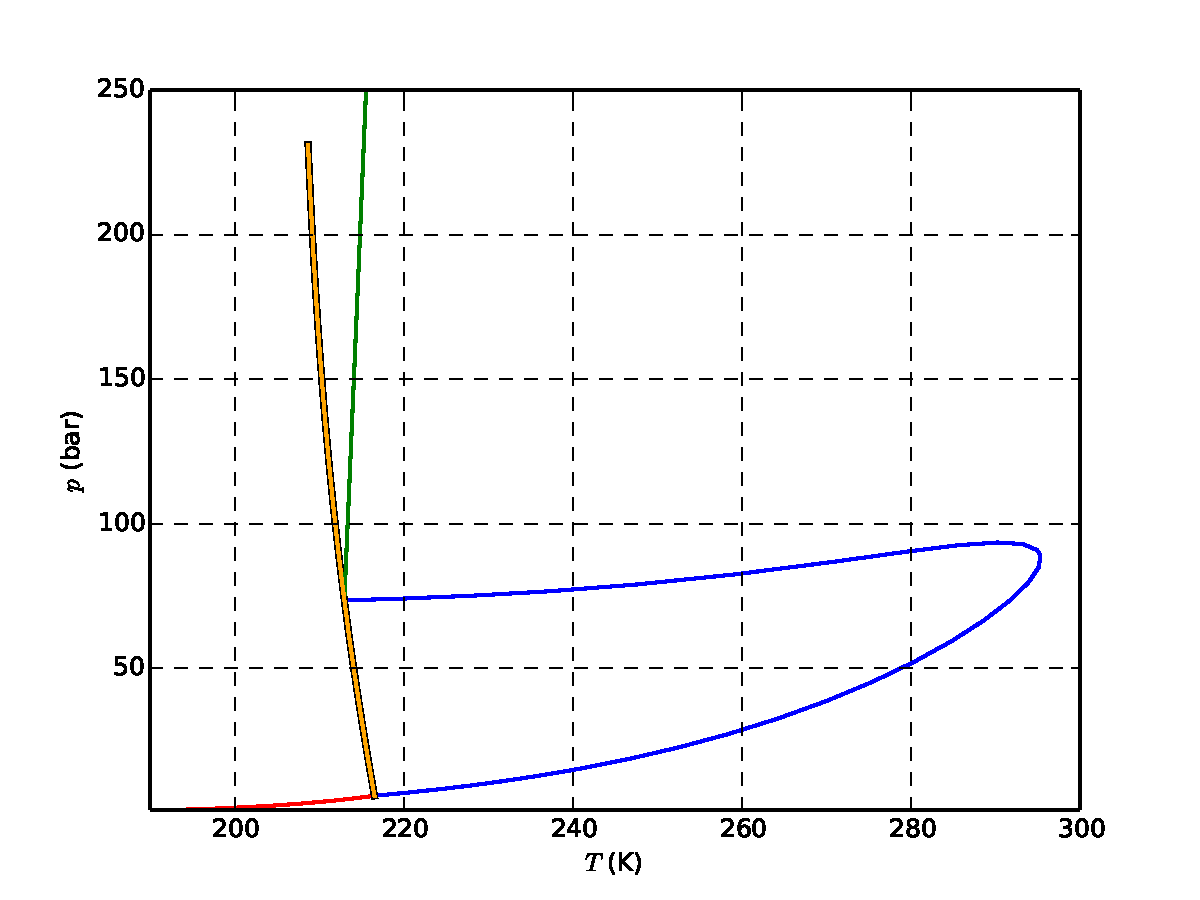
\includegraphics[width=0.9\textwidth]{ptenv}
    \caption{Phase diagram for the temperature--pressure space. The
      blue and the black line encircle the vapor-liquid region. Above
      the red line and left of the orange line we have the vapor solid
      region. The green line is the solid appearance line in from the
      liquid phase. It is seen that there is no three-phase area, only
      a line, as the orange and black line coincide, ending in a
      critical point.}
    \label{fig:ptenv}
  \end{subfigure}
  \hfill
  \begin{subfigure}[t]{0.49\linewidth}
    \centering
    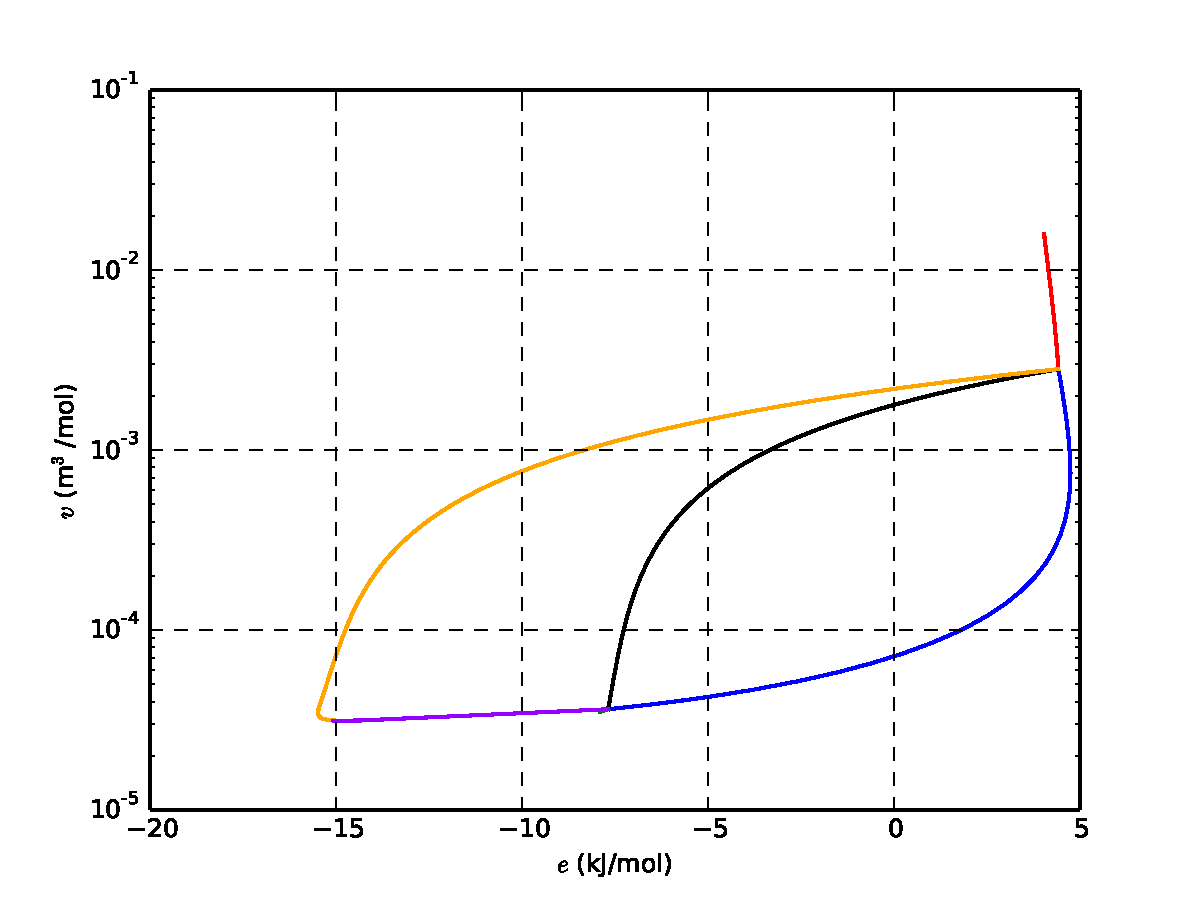
\includegraphics[width=0.9\linewidth]{uvenv}
    \caption{Phase diagram for the internal-energy--volume space.}
    \label{fig:uvenv}
  \end{subfigure}
  \\[12pt]
  \begin{subfigure}[b]{0.49\linewidth}
    \centering
    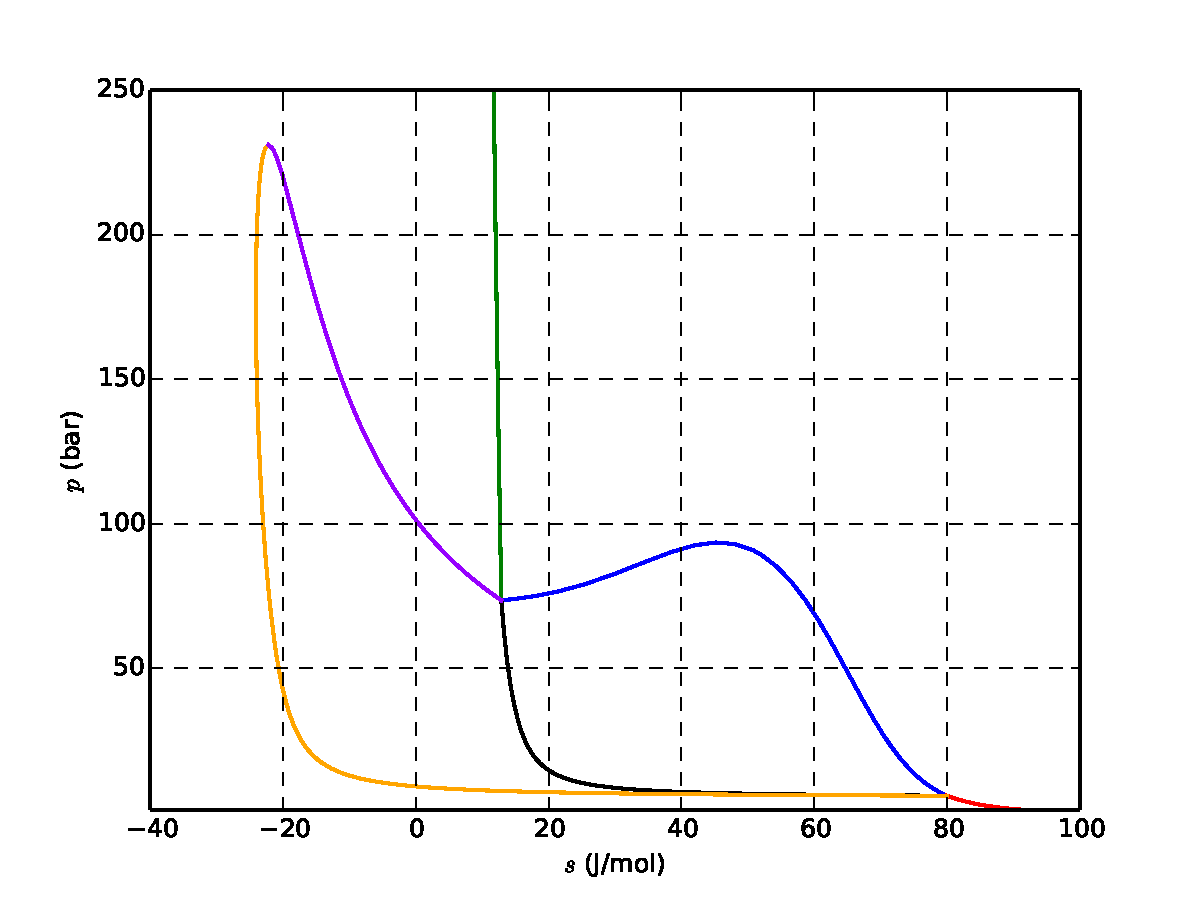
\includegraphics[width=0.9\textwidth]{psenv}
    \caption{Phase diagram for the pressure--entropy space. Here the
      three phase line in the temperature-pressure space represent an
      area enclosed by the black, purple and yellow line. The pressure
      maximum of this region coincide with a critical point.}
    \label{fig:psenv}
  \end{subfigure}
  \hfill
  \begin{subfigure}[b]{0.49\linewidth}
    \hfill
  \end{subfigure}
  \caption{Phase diagrams for a \ce{CO2}-\ce{N2} mixture. The mole
    fraction vector of the mixture is $\left[0.875,0.125\right]$}
  \label{fig:twoCompPhaseDiagram}
\end{figure*}

Here we choose the use of pressure and solid phase fraction. As the temperature is fairly constant along the three-phase line, it is considered better to use pressure. The strategy when solving is to search along the three-phase line, implying that temperature ($T=T(p)$), gas phase composition ($\vektor{Y}=\vektor{Y}(T(p),p)$) and liquid phase composition ($\vektor{X}=\vektor{X}(T(p),p)$) are known from the pressure alone.

\subsection{Three-phase line}

\subsubsection{The UV-flash}
The equations required to calculate the three phase line is given in the envelope memo, and best calculated for $\beta_\sol = 0$. Not that at a given temperature and pressure, changing $\beta_\sol = 0$, do not change the phase composition of the gas or liquid phase.

The enthalpy, specific volume and internal energy of a gas-liquid-solid mixture is described as,
\begin{align}
   h_{\text{mix}} &= \beta_\vap h_\vap + \beta_\liq h_\liq + \beta_\sol h_\sol \label{eq:hmix},\\
   v_{\text{mix}} &= \beta_\vap v_\vap + \beta_\liq v_\liq + \beta_\sol v_\sol \label{eq:vmix},\\
   e_{\text{mix}} &=  h_{\text{mix}} - p v_{\text{mix}} \label{eq:emix}.
\end{align}

Differentiating the mixture enthalpy along the three-phase line, using pressure and solid fraction as variables, yields,

\begin{align}
  \pd{h_{\text{mix}}}{p} &= \pd{h_{\text{mix}}}{p} + \pd{h_{\text{mix}}}{t}\pd{t}{p} + \pd{\left(\beta_\vap h_\vap\right)}{\vektor{n}_\vap}\pd{\vektor{n}_\vap}{p} + \pd{\left(\beta_\liq h_\liq\right)}{\vektor{n}_\liq}\pd{\vektor{n}_\liq}{p} \label{eq:dhmixdp},\\
  \pd{h_{\text{mix}}}{\beta_\sol} &= h_\sol + \pd{\left(\beta_\vap h_\vap\right)}{\vektor{n}_\vap}\pd{\vektor{n}_\vap}{\beta_\sol} + \pd{\left(\beta_\liq h_\liq\right)}{\vektor{n}_\liq}\pd{\vektor{n}_\liq}{\beta_\sol} \label{eq:dhmixdbs}.
\end{align}

The specific volume differentials take the same form. The required differentials along the three-phase line therefore becomes,
\begin{gather}
\ponel{t}{p}{\beta_\sol}, \ponel{\vektor{n}_\vap}{p}{\beta_\sol}, \ponel{\vektor{n}_\liq}{p}{\beta_\sol}, \ponel{\vektor{n}_\vap}{\beta_\sol}{p}, \ponel{\vektor{n}_\liq}{\beta_\sol}{p} \label{eq:tpldiff}
\end{gather}

The envelope solver give the gas phase fraction, $\tilde{\beta}_\vap$, given a zero solid phase $\tilde{\beta}_\sol = 0$. To calculate the real gas (${\beta}_\vap$) and liquid (${\beta}_\liq$) phase fractions, the mass balance for the solid component yields,
\begin{align}
  \beta_\vap &= \frac{Z_{is} - X_{is} +
               \beta_\sol \left( X_{is} - 1\right)}{Y_{is}-X_{is}}, \label{eq:betavap} \\
  \beta_\liq &= 1 - \tilde{\beta}_\vap - \beta_\sol . \label{eq:betabalance}
\end{align}

The relation between mole numbers and mole fractions are as follows,
\begin{align}
  \vektor{n}_\vap &= \vektor{Y}\beta_\vap \label{eq:ng}, \\
  \vektor{n}_\liq &= \vektor{X}\left(1 - \beta_\vap - \beta_\sol\right).
\end{align}

The differentials at constant pressure therefore becomes,
\begin{align}
  \pd{\vektor{n}_\vap}{\beta_\sol} &= \vektor{Y}\pd{\beta_\vap}{\beta_\sol} , \\
  \pd{\vektor{n}_\liq}{\beta_\sol} &= - \vektor{X}\left(\pd{\beta_\vap}{\beta_\sol} + 1\right).
\end{align}
From Equation \ref{eq:betavap} we have,
\begin{equation}
  \pd{\beta_\vap}{\beta_\sol} = \frac{X_{is} - 1}{Y_{is}-X_{is}}.
\end{equation}

The envelope three-phase line lineraisation will provide information on how the temperature, composition and gas phase fraction changes with pressure, ie. $\partial T / \partial \ln p$, $\partial \ln K / \partial \ln p$ and $\partial \beta_\vap / \partial \ln p$. These can be used to construct the required pressure differentials.

The relation between $\vektor{K}$ and $\tilde{\beta}_\vap$ and the gas and liquid composition, are
\begin{align}
  \vektor{X} &= \frac{\vektor{Z}}{1-\tilde{\beta}_\vap+\tilde{\beta}_\vap \vektor{K}}, \\
  \vektor{Y} &= \vektor{K} \vektor{X}.
\end{align}

The differentials of the compositions then become,
\begin{align}
  \pd{\vektor{X}}{K} &= -\frac{\tilde{\beta}_\vap \vektor{Z}}{\left(1-\tilde{\beta}_\vap+\tilde{\beta}_\vap \vektor{K}\right)^2} = -\frac{\tilde{\beta}_\vap \vektor{ X}}{1-\tilde{\beta}_\vap+\tilde{\beta}_\vap \vektor{K}}, \\
  \pd{\vektor{Y}}{K} &= \vektor{X} -\frac{\tilde{\beta}_\vap \vektor{ Y}}{1-\tilde{\beta}_\vap+\tilde{\beta}_\vap \vektor{K}},\\
  \pd{\vektor{X}}{\tilde{\beta}_\vap} &= -\frac{ \vektor{Z}\left(\vektor{K}-1\right)}{\left(1-\tilde{\beta}_\vap+\tilde{\beta}_\vap \vektor{K}\right)^2} = -\frac{\vektor{ X}\left(\vektor{K}-1\right)}{1-\tilde{\beta}_\vap+\tilde{\beta}_\vap \vektor{K}}, \\
  \pd{\vektor{Y}}{\tilde{\beta}_\vap} &= -\frac{\vektor{Y}\left(\vektor{K}-1\right)}{1-\tilde{\beta}_\vap+\tilde{\beta}_\vap \vektor{K}}.
\end{align}

From Equation \ref{eq:ng}, the mole number differentials can be derived,
\begin{align}
  \pd{\vektor{n}_\vap}{p} &= \tilde{\beta}_\vap\left( \pd{\vektor{Y}}{\vektor{K}} + \pd{\vektor{Y}}{\vektor{K}} \right) \pd{\vektor{K}}{p} + \vektor{Y}\pd{\tilde{\beta}_\vap}{p}
\end{align}

\subsubsection{The PS-flash}

The three-phase line must also be treated separately for two-component mixtures. By locating the three-phase line point for the specified pressure, the entropies at $\beta_\sol = 0$, $s_{\left[\beta_\sol = 0\right]}$, and $\beta_\liq = 0$, $s_{\left[\beta_\liq = 0\right]}$, will determine if the solution resides on the three-phase line.

The solid and gas phase fractions at zero liquid phase fraction is found from Equation \ref{eq:betavap} and Equation \ref{eq:betabalance}, when setting $\beta_\liq = 0$,

\begin{align}
  \beta_\sol &= \frac{Z_{is} - Y_{is}}{1 - Y_{is}},\\
  \beta_\vap &= 1 - \beta_\sol .
\end{align}

If the specified entropy , $s_{\text{s}}$, satisfies,
\begin{equation}
  s_{\left[\beta_\liq = 0\right]} \leq s_{\text{s}} \leq s_{\left[\beta_\sol = 0\right]},
\end{equation}
the solution resides on the three-phase line. In this case, the phase fractions must be determined from the following equation,

\begin{equation}
  s_{\text{s}} = \beta_\vap s_\vap + \beta_\liq s_\liq + \beta_\sol s_\sol .
  \label{eq:striple}
\end{equation}

Combining Equation \ref{eq:striple} with the equations \ref{eq:betavap} and \ref{eq:betabalance}, the problem is reduced to solving for $\beta_\sol$,

% \begin{align}
%   s_{\text{s}} &= \beta_\vap s_\vap + \left(1 - \beta_\vap - \beta_\sol\right) s_\liq + \beta_\sol s_\sol ,\\
%   &= \beta_\vap \left(s_\vap - s_\liq\right) + s_\liq + \beta_\sol \left(s_\sol - s_\liq \right) ,\\
%   &=  \frac{\left(s_\vap - s_\liq\right) \left(Z_{is} - X_{is}\right)}{Y_{is}-X_{is}} + \frac{\beta_\sol \left(s_\vap - s_\liq\right) \left( X_{is} - 1\right)}{Y_{is}-X_{is}} + s_\liq + \beta_\sol \left(s_\sol - s_\liq \right) ,\\
%   &=  \frac{\left(s_\vap - s_\liq\right) \left(Z_{is} - X_{is}\right)}{Y_{is}-X_{is}} + s_\liq + \beta_\sol \left[\frac{\left(s_\vap - s_\liq\right) \left(X_{is} - 1\right)}{Y_{is}-X_{is}}  + s_\sol - s_\liq \right].
%   \label{eq:striplebetasol}
% \end{align}

\begin{equation}
  % \beta_\sol &= \frac{s_{\text{s}} - s_\liq - \frac{\left(s_\vap - s_\liq\right) \left(Z_{is} - X_{is}\right)}{Y_{is}-X_{is}}} {\frac{\left(s_\vap - s_\liq\right) \left(X_{is} - 1\right)}{Y_{is}-X_{is}}  + s_\sol - s_\liq }.\\
 \beta_\sol = \frac{\biggl(s_{\text{s}} - s_\liq \biggr) \biggl(Y_{is}-X_{is}\biggr) - \biggl(s_\vap - s_\liq\biggr) \biggl(Z_{is} - X_{is}\biggr)} {\biggl(s_\vap - s_\liq\biggr) \biggl(X_{is} - 1\biggr)  + \biggl(s_\sol - s_\liq \biggr) \biggl(Y_{is}-X_{is}\biggr)}.
  \label{eq:entropy_beta_sol}
\end{equation}

\section{Results}
\label{sec:results}
In order to test the new implementation, TPlib and a
thermodynamic library from {\it Danmarks Tekniske Universitet} (DTU), is
used. This work could therefore be performed in parallel with the new
implementation for the equation of state with mixing rules.

The algorithms are tested on a temperature-pressure grid, for multiple
compositions.
\subsection{Testing \flash{TP}}
The main testing of the \flash{TP}, has been to solve the flash
problem on large temperature-pressure grid, and compare the phase
envelope and results with TPLib. 

Multiple \coto~rich mixtures of \coto-CH$_4$-N$_2$ have been tested.

\subsection{Multiphase \flash{TP}}
The main testing of the multiphase \flash{TP} algorithm has been on
the following two mixtures.
\subsubsection{Test case 1 - Multiphase \flash{TP}}
A 5 component mixture (66\% CH$_4$, 3\% C$_2$H$_6$, 3\% C$_3$H$_8$,
5\% \coto~and 25\% H$_2$S), is selected because it is known to produce multiple phases (LLV, LV and LL).

Figure \ref{fig:LLV5} shows the number of stable phases found for this
test mixtures in the $T\text{-}P$ space.

\begin{figure}[tbp]
  \centering
  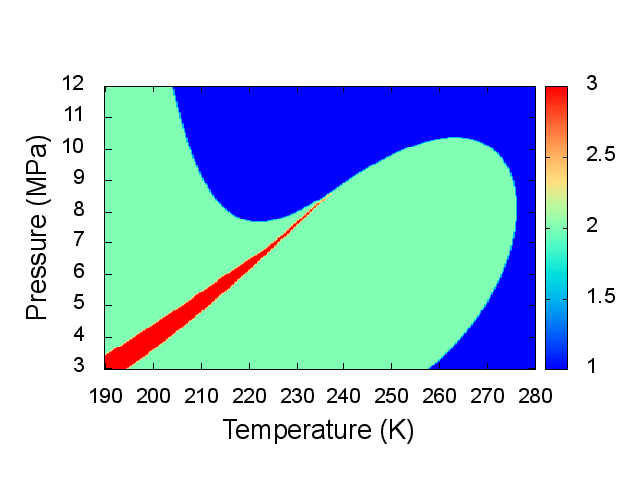
\includegraphics[width=0.8\textwidth]{phase_contour_tp.png}
  \caption{5 component test mixture. The red area is LLV. The blue
    area is single phase. The green area to the left is LL, and the
    other green area is LV.}
  \label{fig:LLV5}
\end{figure}

\subsubsection{Test case 2 - Multiphase \flash{TP}}
A 3 component mixture (5\% CH$_4$,90\% \coto~and 5\% H$_2$O), is
selected because it is known to produce multiple phases (LLV, LV and LL).

Figure \ref{fig:LLV3} shows the number of stable phases found for this
test mixtures in the $T\text{-}P$ space.

\begin{figure}[tbp]
  \centering
  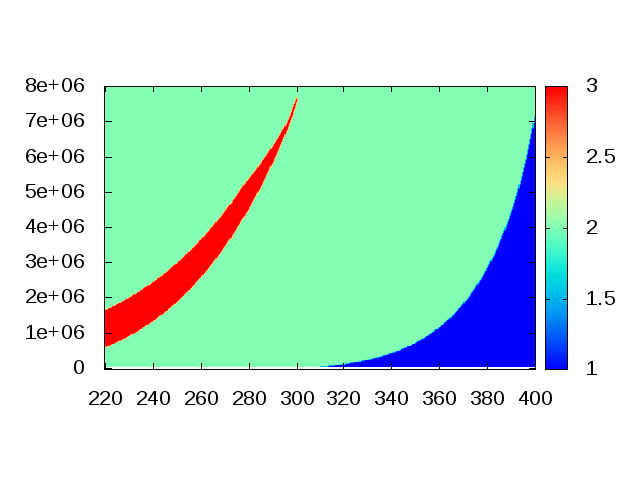
\includegraphics[width=0.8\textwidth]{phase_contour_H2O.png}
  \caption{3 component test mixture. The red area is LLV. The blue
    area is single phase. The green area to the left is LL, and the
    other green area is LV.}
  \label{fig:LLV3}
\end{figure}

\subsection{Testing \flash{HP} and \flash{SP}}
Test prosedure for the \flash{HP} and \flash{SP}:
\begin{enumerate}
\item Perform a \flash{TP}.
\item Calculate enthalpy or entropy.
\item Set a random initial value for the temperature. $120 \ge T_{\text{init}} \ge
  999$ K.
\item Perform a \flash{HP} or \flash{SP}, and compare the resulting
  temperature with the specified temperature.
\end{enumerate}
Multiple \coto~rich mixtures of \coto-CH$_4$-N$_2$ have been tested.

\subsection{Testing \flash{UV}}
Test prosedure for the \flash{UV}:
\begin{enumerate}
\item Perform a \flash{TP}, for ($T^*,P^*$).
\item Calculate internal energy and specific volume.
\item Set an random initial value for the temperature. $T^* - 50 \ge T_{\text{init}} \ge
  T^* + 50$ K.
\item Set a random initial value for the pressure. $P^* - 5e5 \ge P_{\text{init}} \ge
  P^* + 5e5$ K.
\item Perform a \flash{UV}, and compare the resulting
  temperature and pressure  with the specified temperature and pressure.
\end{enumerate}
Multiple \coto~rich mixtures of \coto-CH$_4$-N$_2$ have been tested.

\section{Conclusion and future work}
\label{sec:conclusion}
In this memo, it has been described how state-of-the-art algorithms
for the \flash{TP}, \flash{HP}, \flash{SP} and \flash{UV} have been implemented in the new
flexible thermodynamic workbench developed at SINTEF: ''ThermoPack''. A
new multiphase-flash capable of handling several liquid phases has
also been implemented. The multiphase-flash implementation
successfully predicted the phase diagrams for two relevant mixtures.

Future work for the multiphase-flash will be to validate that it
calculates accurately for other mixtures relevant for CCS, and use it
to predict for which mixtures and temperature, pressure ranges
multiphase systems should be expected. In addition, formation of
solids should be implemented as part of the multiphase-flash. 

Due to improvement of the other flash calculations it is expected that the new \flash{UV} is faster and more
robust than the previous implementation.

%\subsection{\NR~solver}
%To be implemented.

\clearpage

\bibliographystyle{plain}
\bibliography{../thermopack}

%\appendix


\end{document}
%%% Local Variables: 
%%% mode: latex
%%% TeX-master: t
%%% ispell-local-dictionary: "british"
%%% End: 
